%
% ecte457.sty. A very simple style for ECTE457 Thesis reports.
% The process assumed will be tex to pdf.
% 
% Updated to a squeezed up version in 2012.
%
\documentclass[12pt,a4paper,fleqn]{report}
\usepackage{ecte45x}
%
% mmmm, natbib. tastier and better than bibtex or biblatex
\usepackage[sort&compress,square,numbers]{natbib}
%
% for the inclusion of eps and ps graphics
\usepackage{graphicx}
%
% for changing margins for one page
\usepackage{chngpage}
%
\usepackage{setspace}
%
% setup the page margins
\usepackage[left=35mm,right=25mm,top=25mm,bottom=25mm]{geometry}
%
% for tables that need to run over several pages
\usepackage{longtable}
%
% gives you more control of the enumeration lists
\usepackage{enumerate}
\usepackage{paralist}
%
% a better caption for figure and tables. This package will put the figure
% name and number in bold.
\usepackage[labelfont=bf,justification=centering]{caption}
%
% for the LaTeX symbol
\usepackage{latexsym}
%
% for table cells that need to span multiple rows
\usepackage{multirow}
%
% better control over equation arrays
\usepackage{array}
%
% formats URL nicely, especially in the bibliography
\usepackage{url}
%
% if you need a page rotated
\usepackage{lscape}
%
% formats dates and times nicely
\usepackage{datetime}

% Change font size. Used to literature planer. 
\usepackage{sectsty}
\sectionfont{\fontsize{12}{16}\selectfont}

% Makes it able to write text in different colors. 
% Ex; \textcolor{blue}{This is a sample text in blue.}
\usepackage{xcolor}

% Makes it able to comment sections. 
\usepackage{verbatim}


%
% place the chapter title and page number in the header. no footers.
\usepackage{fancyhdr}
%
% titlesec is used to squeeze up some space
\usepackage[compact]{titlesec}
\titleformat{\chapter}[display]{\normalfont\huge\bfseries}{\chaptertitlename\ \thechapter}{0pt}{\Huge}
\titlespacing{\chapter}{0pt}{*-10}{*0}
\titlespacing{\section}{0pt}{*-1}{*-1}
\titlespacing{\subsection}{0pt}{*-1}{*-1}
\titlespacing{\subsubsection}{0pt}{*-1}{*-1}
%
% squeeze some more space around equations
\makeatletter
\g@addto@macro\normalsize{\setlength\abovedisplayskip{0pt}}
\g@addto@macro\normalsize{\setlength\belowdisplayskip{0pt}}
\g@addto@macro\normalsize{\setlength\abovedisplayshortskip{0pt}}
\g@addto@macro\normalsize{\setlength\belowdisplayshortskip{0pt}}
\makeatother
%
% squeeze some bibliography space
\setlength{\bibsep}{0.0pt}
\setlength{\bibhang}{0em}
\def\bibfont{\footnotesize}
%
% nicer looking tables
\setlength\extrarowheight{2pt}
%
% you need to place your details here so the title page and statement of
% originality are correctly created.
%
\degreetitle{Bachelor of Engineering (Electrical), Bachelor of Mathematics}
\submitdate{June, 2013}
% Don't forget the proper title for your supervisor.
\supervisor{Dr John Smith}
\title{The Title of My Thesis}
\author{Joe E. Blogs}
\studentid{1234567}
%
% establish the fancy headers to be used throughout the document
\rhead{\thepage}
\lhead{\nouppercase{\leftmark}}
\rfoot{}
\cfoot{}
\lfoot{}
%
% Begin the document.
%
\begin{document}
%
% Change the filenames to whatever you have chosen for your project.
%
% The "beforeabstract" macro essentially creates the title page from the data
% you include in the preamble of this document.
%
\beforeabstract
%
% The first content will be the abstract.
%


\tocsection{Abstract}
\label{abstract}
According to some people, the abstract should be
approximately 300 words, and no more than 700 words. It should be an
`Informative Abstract'.



\tableofcontents
\listoffigures
\listoftables

%
% Any acknowledgements you might wish to include. Acknowledgements should use
% the "notocsection" environment (so it doesn't get included in the table of
% contents). See acknowledgements.tex.
%
\notocsection{Acknowledgements}

I would like to thank the Flying Spaghetti Monster for his guidance and
constant inspiration \ldots

%
% The "afterabstract" macro creates the statement of originality, table of
% contents, list of tables and list of figures.
%
\afterabstract
%
% Symbols and abbreviations go after the contents, list of figures and list
% of tables. The glossary should use the "tocssection" environment (so it
% appears in the table of contents). See glossary.tex.


\tocsection{Abbreviations and Symbols}
\label{glossary}
\begin{singlespacing}
\begin{longtable}{p{0.15\textwidth} p{0.85\textwidth}}
$g$ & Airgap, mm\\
$g_e$ & Equivalent airgap, mm\\
$J$ & Current Density, amps/metre\\
$L_R$ & Rotor stack length, mm\\
$N_s$ & Number of Slots per Pole Pair\\
$\theta_m$ & Mechanical angle, radians\\
$\theta, \theta_e$ & Electrical angle, radians\\
$\theta_p$ & Pole Arc angle, radians\\
$p$ & Pole pairs\\
$R$ & Stator radius, mm\\
$\Re_l$ & Leakage Reluctance, amps/weber/metre\\
$\Re$ & Reluctance amps/weber\\
$\mu_o$ & Permeability constant, $4\pi \times 10^{-7}$ amps/metre\\

\end{longtable}
\end{singlespacing}




%
% The table that describes your list of changes from ECTE451 to ECTE458. You
% need only include this section when submitting your ECTE458 report. If this
% is your ECTE451 report, comment out (%) or remove the following \include.
%
%%\tocsection{List of Changes}
\begin{singlespacing}
\begin{tabular}{|c|p{10cm}|p{2cm}|}
\hline
\textbf{Section}&\centering{\textbf{Statement of Changes}}&\centering{\textbf{Page Number}}\tabularnewline
\hline
Abstract& Complete re-write because the abstract that was produced for Autumn
session was complete nonsense.&\centering{\pageref{abstract}}\tabularnewline
\hline
Glossary&Changed to single spacing instead of
double&\centering{\pageref{glossary}}\tabularnewline
\hline
\ref{chap:first}&Included a blurb about how this is a new version
of the ECTE45x style etc.&\centering{\pageref{chap:first}}\tabularnewline
\hline
References&Using a 10pt font and various other space-saving
features.&\centering{\pageref{refs}}\tabularnewline
\hline
&  &  \\
&  &  \\ 
\hline
&  &  \\
&  &  \\ 
\hline
&  &  \\
&  &  \\ 
\hline
&  &  \\
&  &  \\ 
\hline
&  &  \\
&  &  \\ 
\hline
&  &  \\
&  &  \\ 
\hline
&  &  \\
&  &  \\ 
\hline
\end{tabular}
\end{singlespacing}

%
\pagenumbering{arabic}
\pagestyle{fancy}
%
% Now go through and input the bulk of the thesis.
%
\chapter{The First Chapter}\label{chap:first}

\section{Physical rehabilitation}
\section{Perturbation devices}
\section{Exoskeleton (Rehabilitation)}
Rehabilitation system tend to be not used if the setup takes mode than 5 minutes. Hence, the system needs to be easy to use and fast to set up.  
\section{Actuators and transmissions the exoskeleton devices}
Article; A survey on robotic devices for upper limb rehabilitation. chapter; Actuators and transmissions

\begin{comment}


\section{Reffs}
\cite{NEUROExos}
\cite{shapeMemoryAlloy}
\cite{rahman2019review}
\cite{rahman2015emg}
\cite{moura2016exoskeleton}
\cite{maciejasz2014survey}
\cite{blank2014current}
\cite{khan2017neurorehabilitation}
\cite{geurts2005review}
\cite{rehmat2018upper}
%11
\cite{Schorsch2014}
\cite{sEMG-based2019}
\cite{lu2019development}
\cite{sridar2017development}
\cite{tuatulea2019mechanical}

%16
\cite{thoroughman1999electromyographic}

% Thomas 
\cite{evison2016design}
\end{comment}
\chapter{Early research} \label{chap:research}

\section{Exoskeleton design}
In this section the different thoughts and research will be noted and explained. 

\subsection{Bicep size}
The bicep average size was found in this research paper:| Anthropometric Reference Data for Children and Adults: United States, 2011–2014



\chapter{Notes and Ideas}



\section{To research}
\begin{enumerate}
    \item Functional Electrical Stimulation (FES)
    \item will this be a Haptic device
    \item Exoskeleton history, why when. 
    \item Balance and recovery. 
    \item Investigate previous designs. 
    \item Forces generated by an elbow
    \item Forces the elbow can handle.
    \item Rotation in elbow joint.
    \item Best suited material.
    \item Best electrical components. Actuator, sensor and battery. 
    \item Servo motor vs Steppe vs something else? Servo motors might be the best option due to it high torque at high speeds. In addition it is already made to be controlled to a given set of angles. 
    \item Damping effect of the human body. 
    \item Control strategy. 
    
\end{enumerate}{}
\subsection{Limitations and requirements}
\begin{itemize}
    \item Elbow max-min Angel. 0 -120
    \item Movement frequency.
    \item Actuator max-min torque.
    \item Minimize weight. 
    
\end{itemize}{}


\section{Ideas}
\begin{itemize}
    \item Using soft robotics? (maybe not) 
    \item Wire translation.
    \item Solenoid clutch 
    \item Servo motor vs Steppe vs something else? 
    \item alu profile for with adjustments 
    \item Reimdrift.
    \item Closed loop control, flex, EMG, Load-cell, 6-10 dof. 
    \item laser scan an arm for fitness? 
    \item Magnetic fluids??? 
    \item USB C charging
    \item The actuator should be placed as high on the arm as possible to avoid the additional weight. 
    \item Adjustable size. 
    \item Measuring EMG, torque, angle and load-cell. 
    
\end{itemize}{}

\section{Questions}
\begin{enumerate}
    \item Shall i use a innovation and design method? 
    \item User interface? Online? 
    \item EMG sensor. 
\end{enumerate}{}



\section{Links}
\subsection{EduExo elbow kit}
The EduExo elbow is a DIY exoskeleton elbow project. \newline
https://all3dp.com/eduexo-exoskeleton-kickstarter/

\subsection{EMG Sensors}
\subsubsection{Sparkfun}
https://www.sparkfun.com/products/13723

\subsection{Exoskeleton (Robotics)}
https://www.sciencedirect.com/topics/engineering/exoskeleton-robotics

\subsection{Red Green LED}
https://protostack.com.au/shop/led-lcd/3mm/led-red-green-3mm-common-cathode-diffused/

\subsection{Stain Gauge}
https://www.kyowa-ei.com/eng/product/category/strain\_gages/order/index.html

\subsection{Feste for robot}
https://www.ebay.com.au/itm/Elbow-Brace-Compression-Exercise-Pressed-Sport-Dropship-Fashion-Lightweight-LS/352970716105?hash=item522eb1b3c9:g:FG8AAOSwlThdNQ5p
\newline
https://www.aliexpress.com/item/32877777311.html?spm=a2g0o.detail.1000023.8.11ff5fcexRPcXj
\newline
% https://tynor.com.au/products/rom-elbow-brace?variant=7124780417082&currency=AUD&utm_campaign=gs-2018-11-10&utm_source=google&utm_medium=smart_campaign&gclid=Cj0KCQjwjoH0BRD6ARIsAEWO9DsXc-JRCDdGqUsaJaJRPgHv3hrBqVHF6bR8L5mHxZl_XFgWqcu0RV0aAg9qEALw_wcB

Overall Length : 36 cm (l) | Length below Elbow : 19 cm + above Elbow : 16 cm | Extension : 0 to 90 degrees , Flexion : 0 to 120 degrees | Maximum circumference : 40 cm (at arm) + 35 cm (forearm) | Velcro Strap : 2 Arm + 2 Forearm | Shoulder strap

https://www.orthomen.com/products/rom-arm-elbow-brace
\chapter{Design and design notes}

\section{Actuator selection}
There is many different types of actuators used in exoskeletons. The most common once are pneumatic, hydraulic and electrical \citep{maciejasz2014survey}. Hydraulic actuator is commonly used for high power application such as military and industrial lifting. Electrical motors is the most popular actuator in the field of rehabilitation. This is mainly due to it high controllability and high position accuracy. Light weight batteries can be used as the energy source providing flexible and mobile systems. [ROBOT Book]

To be able to select an appropriate motor, several factors need to be evaluated. The most important is the torque force(Unknown) and speed (>2.066 rad/s | > 120deg/s), then the weight, size and the price.

(Servo vs stepper vs dc motor) 

Linear transition? 

\subsection{Actuator for this thesis}
Since this project is based on a previous one, some motors have all ready been purchased and tested. And since the accurate value for the needed torque is hard to obtain, the MX-28 motor will be used for the first prototype. From the litterateur it can be found that the muscle reflex can provide everything between. 


\section{Sensor selection}
1. Dynamic, 2. Kinematic, 3. Trigger signals. 
Most exoskeleton require a some sensor feedback to control the force, torque and angle of the device, and some actuators has these sensors integrated. But since the link between the body and the device usually is not absolutely rigid, additional sensors can be used to improve the system response time [Thomas]. This is especially critical for person-in-control applications where the user should not experience any resistance from the device. Thomas Evison and others [kilder] have used dynamic signals to improve the performance of the controller by measuring the instant change of movement and use it as the controller input. It has been proven that such a closed loop controller can significantly decrease the system impedance. Some commonly used sensors is load-cells, EMG sensors and force sensors. 

Kinematic signal is also important for accurate position control.
With sensor is the best suited for angular measuremnt.
 \textcolor{red}{TODO}

\subsection{This thesis}
For this thesis the MX-28 electrical motor is likely to be used. This has all ready an potenitimeter implemented. 



\section{Control}



\section{Design method}
% Soft vs Rigid
One of the major challenges in exoskeleton development is weight.  Hence, it is important to select the correct material. Depending on the application, the materials used in such devices vary. One way of designing exoskeletons is with a soft bodies. These designs have the advantage of being light weighted and comfortable to wear \cite{sEMG-based2019, lu2019development, sridar2017development}. However, it is hard to attach actuators and sensors to the soft exoskeleton it self, and consequently the complexity of the system will increase. Another and more common way of design is the rigid exoskeletons. It is usually made with a steel, aluminium, titanium or carbon fibre body to make it strong and stable. Titanium and carbon fibre provides the best strength-to-weight ratio, but it is more expensive than the others. Therefore, aluminium is the most popular choice since it has a relatively good weight-to-strength ratio and is fairly cheap. For being able to attach the device to the human body, plastic or similar material is used to provide a flexible fit of the exoskeleton. [Kilde] 

\subsection{Material}
Compare PLA, ABS And Carbon filament in therms of flexibility, durability and strength.


\begin{table}[h!]
\centering
\begin{tabular}{|c|c|}
\hline
\textbf{Application} & \textbf{Material} \\ \hline
Joint/Frame & Aluminum \\ \hline
Fit prototype & Plastic (ABS) \\ \hline
Fit later design & Carbon? \\ \hline
Comfort & Neoprene? \\ \hline
\end{tabular}
\end{table}

\section{Notes and summaries}
\begin{itemize}
    \item Electric actuators will be used due to it angular accuracy. 
    \item 
    \item 
\end{itemize}{}


\section{Design measurements}
According to ANTHROPOMETRY AND MASS DISTRIBUTION FOR HUMAN ANALOGUES, the different average measurement of different body parts is: 
\begin{table}[h!]
\centering
\begin{tabular}{|c|c|c|c|}
\hline
\textbf{Body part} & \multicolumn{3}{c|}{\textbf{Measurement (mm)}} \\ \hline
Size & S & M & L \\ \hline
Forearm Circumference & 265 & 285 & 302 \\ \hline
Upper Arm Circumference & 284 & 313 & 337 \\ \hline
Wrist Circumference & 167 & 177 & 187 \\ \hline
Forearm Length &  &  &  \\ \hline
Upper arm langth &  &  &  \\ \hline
\end{tabular}
\end{table}



\section{Actuation method and transition}
Research pros and cons of belt driven, gear and 

https://www.jospt.org/doi/pdf/10.2519/jospt.1997.25.6.395 \newline

https://itstillruns.com/calculate-gear-ratios-torque-8140164.html \newline

\section{Evaluation of previous design}


\section{Elbow Torque and Angular Velocity}
\subsection{Bio dynamics Founder}
Hill model: 

\subsection{Reffs}
\begin{enumerate}
    \item Monitoring elbow isometric contraction by novel wearable fabric sensing device.
\end{enumerate}{}
\begin{figure}[h!]
    \centering
    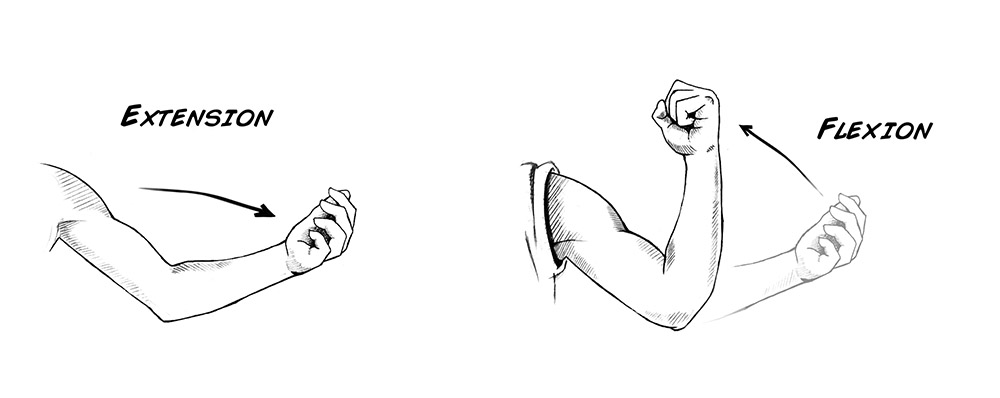
\includegraphics{compact-template/Fig/flexextend.jpg}
    \caption{Flexion and Extraction}
    \label{fig:flexextend}
\end{figure}{}


\section{Balance and recovery research}
\subsection{Center of pressure (COP)}
\textcolor{blue}{TO READ LATER} \newline
In the book Proximal-to-Distal Sequencing Behavior chapter 10, the theory of center of pressure (COP) is explained. This talks about how the human body transfers pressure to the ground to keep balanced. In addition this chapter contains an MatLab example of how to calculate the center of gravity for a moving body based on the measurements from a force plate. 




%
% Use the ieee bibliography style. The bibliography source (database,) in this
% case, is in the file thesis.bib, but of course you can use your own
% filename. 
%
\bibliographystyle{unsrtnat}
\addcontentsline{toc}{chapter}{References}
\bibliography{thesis}
\label{refs}
%
% Include the appendices.
%
\appendix


\chapter{Literature Planner}
%1
\section{NEUROExos: A Powered Elbow Exoskeleton for Physical Rehabilitation}
\textbf{Authors:} Nicola Vitiello, Tommaso Lenzi, Stefano Roccella, Stefano Marco Maria De Rossi, Emanuele Cattin, Francesco Giovacchini, Fabrizio Vecchi and Maria Chiara Carrozza. \newline
\textbf{Publication:} IEEE Transactions on Robotics.  
\textbf{Type:} Journal (Primary) \newline
\textbf{Year Published:}  2013.   
\textbf{Citations:} 141 (scopus) \newline 
\textbf{Publication Rating:}    
\textit{CiteScore:} 9.53. \textit{Rank:} \#3/233 \textit{Percentile:} 98th \newline
\textit{CiteScore Year:} 2018
\textit{In-Category:} Control and Systems Engineering

\textbf{What was the research question?} . 
Can an safe exoskeleton elbow be designed and used in human rehabilitation with a minimum interference of the natural movement. 

\textbf{What themes were discussed in the Literature Review?} 
The team developed and tested an exoskeleton elbow to be used to physical rehabilitation. Their main focus was to rehabilitate people suffering from stroke after effects. The researched had three main focuses. Firstly, it had to be comfortable  and light weighted. Secondly, the design needed to be able to fit different people with different sized arms, and at the same time be adjusted according to the 4DoF of the human elbow. Finally, the elbow needed to be able to used by the patient with a minimal torque interference. At the same time, a different mode should add torque for the movement for the rehabilitation to work. 

\textbf{Design:}  
This thesis is an experimental design where the team have performed different tests to figure out what is the best way of make the elbow. A large part of the mechanical design and concept testing had been done in an earlier article. Firstly, they designed and build the prototype based on knowledge about the elbow limitations and ideal setup. Secondly they designed a controller for operating the arm. 

\textbf{What was the finding?} 
The researches made an elbow where the part connected to the arm was divided in to two layer, one is designed for stiffness while the other is for comfort and fit. Then they made the elbow adjustable with a 4-DOF Mechanism to ensure a perfect alignment to the individual humans elbow. Finally the designed a controller with could work in two modes, \textit{patient-in-control} and \textit{robot-in-control}. The end result show that such an arm can be used to rehabilitate human elbow and it is a safe alternative. 

\textbf{What were the gaps?}   
The device is not suitable for a clinical setting and it is very complex and bulky. 

%2
\section{Wearable elbow exoskeleton actuated with Shape Memory Alloy in antagonist movement}
\textbf{Authors: D. Copaci, D. Blanco, L. Moreno}  \newline
\textbf{Publication:} Biosystems and Biorobotics 
\textbf{Type:} Book Chapter (Primary)  \newline 
\textbf{Year Published: } 2017  
\textbf{Citations:} 5 (scopus) \newline 
\textbf{Publication Rating:}    
\textit{CiteScore:} 0.45. \textit{Rank:} \#437/583 \textit{Percentile:} 24th. \newline
\textit{CiteScore Year:} 2018
\textit{In-Category:} Mechanical Engineering

\textbf{What was the research question?}
Can Shape Memory Alloys be used as actuators if exoskeleton products to reduce weight? 

\textbf{What themes were discussed in the Literature Review?} 
This research are investigating if hydraulic or pneumatic actuation can be used for exoskeleton elbow. A low weight exo elbow is developed to utilize SMA mechanics as actuators. 

\textbf{Design:}  
The article is a experimental design divided in to three parts. Introduction to the problem, methodology, and a chapter about the parallel four-term bilinear PID controller. 

\textbf{What was the finding?} 
The paper found that an exoskeleton elbow can be made utilizing SMA as the actuation source. In addition, this setup made the exo noiseless which might be beneficial in multiple applications. 

\textbf{What were the gaps?}  
The performance of the device is not well described and tested. 

%3
\section{EMG Based Control of a Robotic Exoskeleton for Shoulder and Elbow Motion Assist} 
\textbf{Title of Article:} EMG Based Control of a Robotic Exoskeleton for Shoulder and Elbow Motion Assist \newline     
\textbf{Authors:} Mohammad H. Rahman, Cristobal Ochoa-Luna, and Maarouf Saad and Philippe Archambault.
\textbf{Publication:} Journal of Automation and Control Engineering
\textbf{Type:} Journal (Primary) \newline
\textbf{Year Published:} 2015
\textbf{Citations:} 26 (scopus)
 \textbf{Publication Rating:} NA

\textbf{What was the research question?} 
Can an controller for exoskeleton arm be designed for active control  utilizing EMG sensor as it only input. 

\textbf{What themes were discussed in the Literature Review?} 
This research is based on previous research where an exoskeleton robot is was designed for physical rehabilitation purposes. This robot was designed to control the shoulder, elbow, forearm and wrist motions of a human arm.  The themes discussed in this research is; EMG sensors, measuring of the muscles with EMG sensors, control of exo arms using EMG sensors (ETS-MARSE) and general physical rehabilitation.  

\textbf{Design:}  
This research is an experimental article where the robot is designed in a previous research. This research measures the activity of the muscles on a healthy test subject and then designs a controller for the arm. The controller is then implemented and tested on the same subject. 

\textbf{What was the finding?} 
The research shows that the ETS-MARSE controller can be used for active assistance for the test subject. 

\textbf{What were the gaps?}   
The research team never explains why this type of control is important for rehabilitation purposes. Secondly, the ETS-MARSE work-space is designed with forearm and wrist axis. This axis is not included in to the research. 

%4
\section{A Review of Upper Limb Rehabilitation Robot} 
\textbf{Authors:} Sulaiman Mazlan, Hisyam Abdul Rahman, Dirman Hanafi \newline
\textbf{Publication:} Journal of Tomography System and Sensor Application
\textbf{Type:} Journal (Secondary) \newline
\textbf{Year Published:} 2018
\textbf{Citations:} NA \newline 
\textbf{Publication Rating:} NA 

\textbf{What was the research question?}
Which aspects should future research focus on when it comes to upper limb rehabilitation robots.

\textbf{What themes were discussed in the Literature Review?}  
The research addresses the three main category of end-effector based rehabilitation robots; robot for manipulation, robot for reaching and robot for manipulation and reaching. It also discuss the importance of the rehab robots. Then the paper analyses a total of eighth different robots from the three categories. 

\textbf{Design:}  
A review of different end-effector based rehabilitation robots. 

\textbf{What was the finding?} 
The main findings is that to make a good rehabilitation robot, the complexity will be increased. As a result, the price will rise and the safety decreased. 

\textbf{What were the gaps?}   
The devices functionality is limited and it would be beneficial to add more to accelerate the rehabilitation. 



%5
\section{Exoskeleton application to assist learning of a coincident timing motor task of the arm using passive mechanical perturbations} 
\textbf{Authors:} R.T. Moura, R.S. Souza, E. Garcia, V.H. Quadrado, M.B. Villalpando and A. Forner-Cordero \newline
\textbf{Publication:} EMBS International Conference on Biomedical Robotics and Biomechatronics
\textbf{Type:} Conference Paper \newline
\textbf{Year Published:} 2016 
\textbf{Citations:} 2 (scopus)
\textbf{Publication Rating:} NA    

\textbf{What was the research question?} 
Can the combination virtual reality and mechanical perturbations improves or accelerates motion learning or rehabilitation? 

\textbf{What themes were discussed in the Literature Review?} 
This article have developed and exoskeleton elbow which is able to add perturbations loads to the arm. Then the arm was mounted on to a healthy test subject. The subject was supposed to reach a goal virtual goal displayed on a screen. The main theme is physical rehabilitation of a humans motor control. 

\textbf{Design:}  
The report is an experimental design where the experiments was well planned in advanced. Then the experiments was tested and data collected. In the end of the article the data was analysed. 

\textbf{What was the finding?} 
The researches found that the experimental setup can be used to accelerate the motor learning of a human by controlling the additional load of the arm. 

\textbf{What were the gaps?}   
 The load was static during each reaching test. This perturbation pattern might not be enough to speed up the learning process. 
 Unpredictable perturbations. 


%6
\section{A survey on robotic devices for upper limb rehabilitation.} 
\textbf{Authors:} Maciejasz, Pawe{\l} and Eschweiler, J{\"o}rg and Gerlach-Hahn, Kurt and Jansen-Troy, Arne and Leonhardt, Steffen \newline
\textbf{Publication:} Journal of NeuroEngineering and Rehabilitation
\textbf{Type:} Review \newline
\textbf{Year Published:} 2014
\textbf{Citations:} 446 (scopus) \newline 
\textbf{Publication Rating:}    
\textit{CiteScore:} 4.59 \textit{Rank:} \#2/110  \textit{Percentile:} 98th  \newline
\textit{CiteScore Year:} 2018
\textit{In-Category:} Rehabilitation.

\textbf{What was the research question?} 
What is the pros and cons about the existing designs for upper limb physical rehabilitation purposes? And where should future work focus? 

\textbf{What themes were discussed in the Literature Review?}   
This research is covering upper limb rehabilitation system. In the literature review they analysed 120 different types of systems such as end-effector and exoskeleton system. Then they discussed the different actuators used, sensor used and control methods. In addition, the paper explains why these devises are important and what injuries they can help recover in the future. 

\textbf{Design:}  
This is a review of 120 different system. The systems are divided in to categories based on their limb focus area. 

\textbf{What was the finding?} 
The use of rehabilitation robots for upper limb recovery clearly has a potential in the market. However, it is only the wast majority of the analysed products with has proven to be sustainable and can be used in the medical industry up to this date. This is mainly due to complex systems which is hard to use and set up. Hence, the many of the product is not used. Rehabilitation system tend to be not used if the setup takes mode than 5 minutes. Hence, the system needs to be easy to use and fast to set up. To avoid any injuries, it is important to adjust the exoskeleton robot to the human arm.  

\textbf{What were the gaps?}   
The gap purposed by the researchers is to look to the all ready existing solutions and find ways to improve them in therm of complexity. 

%7
\section{Current Trends in Robot-Assisted Upper-Limb Stroke Rehabilitation: Promoting Patient Engagement in Therapy.} 
\textbf{Authors:} Blank, Amy A and French, James A and Pehlivan, Ali Utku and O’Malley, Marcia K. \newline
\textbf{Publication:} Current Physical Medicine and Rehabilitation Reports
\textbf{Type:} Review \newline
\textbf{Year Published:} 
\textbf{Citations:} 71 (Springer) \newline 
\textbf{Publication Rating:} NA   

\textbf{What was the research question?}
What are the current trends in the field of upper limb Stroke rehabilitation. 

\textbf{What themes were discussed in the Literature Review?}  
Why and how rehabilitation can improve the life quality of a person. Also it discuses why robotic rehabilitation devices seems to have an advantage over traditional physical therapy. 

\textbf{Design:}  
The review have investigated in different upper limb therapy methods and compared them. 

\textbf{What was the finding?} 
The review have found that robotic rehabilitation devices might be a great contribution in the field due to its ability to perform repetitive and intensive rehabilitation at e lower cost. It also found that robots can provide good Assistance-If-Needed controllers. 


\textbf{What were the gaps?} 
The Assistance-If-Needed controllers should be improved to make a personal controller making the rehabilitation method adapt to the patients needs. Also, the majority of exoskeleton arms is heavy. This is often due to heavy actuators.

% 8
\section{Neurorehabilitation: applied neuroplasticity} 
\textbf{Authors:} Khan, Fary and Amatya, Bhasker and Galea, Mary P and Gonzenbach, Roman and Kesselring, J{\"u}rg  \newline
\textbf{Publication:} Journal of Neurology
\textbf{Type:} Journal \newline
\textbf{Year Published:} 2017
\textbf{Citations:} 13 (Scopus)\newline 
\textbf{Publication Rating:}    
\textit{CiteScore:} 3.21  \textit{Rank:} \#64/334 \textit{Percentile:} 80th  \newline
\textit{CiteScore Year:} 2018
\textit{In-Category:} Neurology (clinical)

\textbf{What was the research question?} . 
Will new methods of physical therapy and psychological intervention help in the process of neural rehabilitation after stroke, MS and others diseases. 

\textbf{What themes were discussed in the Literature Review?} 
This literature review talks about the magnitude of the neurological disorders around the world and why it can be hard to deal with such conditions. Then, it explains about neuroplasticity and earlier research proving that it works in many cases. 

\textbf{Design:} 
The article are doing a systematic review on 78 different publication regarding four different neurological conditions: stroke, MS, TBI and PD. Then they check the quality of evidence to see it the publication is reliable or not. 

\textbf{What was the finding?} 
It is clear to say that physical rehabilitation and training has a impact on stroke rehabilitation. However, to be sure that the different methods actually works, scientist need to get under the sell and understand why it works. 

\textbf{What were the gaps?}   
More effort should be up in to MDR and educate and empower patients.
 

% 9
\section{A review of standing balance recovery from stroke} 
\textbf{Authors:} Geurts, Alexander CH and de Haart, Mirjam and van Nes, Ilse JW and Duysens, Jaak. 
\textbf{Publication:} Gait and Posture
\textbf{Type:} Review \newline
\textbf{Year Published:} 2005
\textbf{Citations:} 263 (scopus) \newline 
\textbf{Publication Rating:}    
\textit{CiteScore:} 2,65  \textit{Rank:} \#11/110  \textit{Percentile:} 90th  \newline
\textit{CiteScore Year:} 2018
\textit{In-Category:} Rehabilitation.

\textbf{What was the research question?} 
What is the best method for natural recovery after the balance is damaged due to stroke. 

\textbf{What themes were discussed in the Literature Review?}    
How stroke impact activity of daily living (ADL) and how it impacts the postural control. Also, the different between Unperturbed and perturbed stance and two tree other methods where evaluated. 

\textbf{Design:}  
Each method was analysed individually to investigate if they can be used for balance rehabilitation. 

\textbf{What was the finding?} 
At this point the researchers can not conclude with is the best approach. But, many research papers states that the methods can be used in rehabilitation in the future. 

\textbf{What were the gaps?}   
The different methods needs to be further examined to determine which one is the best. 



% 10
\section{Upper limb rehabilitation using robotic exoskeleton systems: a systematic review} 
\textbf{Authors:} Rehmat, Naqash and Zuo, Jie and Meng, Wei and Liu, Quan and Xie, Sheng Q and Liang, Hui.  \newline
\textbf{Publication:} International Journal of Intelligent Robotics and Applications.
\textbf{Type:} Journal (Secondary) 
\textbf{Year Published:} 2018
\textbf{Citations:} 10 (scopus) \newline 
\textbf{Publication Rating:}  NA  

\textbf{What was the research question?} 
This paper intend to review existing exoskeleton robots for physical rehabilitation and create a reliable guidance for future research.  

\textbf{What themes were discussed in the Literature Review?}    
This research describes the impotence of stroke rehabilitation and how robots can be used in this field. If focuses on the upper limb robots where the two main types are the end effector and the upper exoskeletons. 

\textbf{Design:}  
This is a review where the researchers have analysed different upper limb exoskeleton rehabilitation robots according to their mechanism design, control strategies and clinical trial performance. A table was made holding information about how effective they are. 

\textbf{What was the finding?} 
This paper found that exoskeleton robots with a dedicated control strategy performs better in rehabilitation that those who do not. It was also found that the majority of patient preferred the robotic therapy over the traditional one.   

\textbf{What were the gaps?}   
Only a few on the reviewed paper have collected sufficient feedback from the patients before and after their therapy session. Hence, the fact that parents prefer robots in therapy can not be clearly stated.   


% 11
\section{A novel self-aligning mechanism to decouple force and torques for a planar exoskeleton joint} 
\textbf{Authors:} Schorsch,J. F. and Keemink,A. Q. L. and Stienen,A. H. A. and Van Der Helm,F. C. T. and Abbink,D. A. \newline
\textbf{Publication:} Mechanical Sciences
\textbf{Type:} Journal \newline
\textbf{Year Published:} 2014
\textbf{Citations:} 5 (scopus) \newline 
\textbf{Publication Rating:}    
\textit{CiteScore:} 1.92 \textit{Rank:} \#23/80 \textit{Percentile:} 71th \newline
\textit{CiteScore Year:} 2018
\textit{In-Category:} Fluid Flow and Transfer Processes.

\textbf{What was the research question?}
Can a self aligning exoskeleton be designed so to revile the muscle and joint while force is applied to the users hand. 

\textbf{What themes were discussed in the Literature Review?}   
It explains about tree of the different aligning method of exoskeletons; Manual adjustment, compliant mechanisms, and kinematic redundancy.

\textbf{Design:}  
This paper explains the different method and then designs a theoretical model of an exoskeleton self adjusting joint. 

\textbf{What was the finding?} 
The team found that it is possible to make an exoskeleton which  theoretically carries all the force presented to the users outer arm.  

\textbf{What were the gaps?}   
Even though the maths seems to be correct it is only a theoretical approach. Hence, it is not proven to work physically. 


%%%%% 12
\section{Design and Fuzzy Sliding Mode Admittance Control of a Soft Wearable Exoskeleton for Elbow Rehabilitation} 
\textbf{Authors:} Lu,L. and Wu,Q. and Chen,X. and Shao,Z. and Chen,B. and Wu,H.  \newline
\textbf{What was the research question?}
How can a intelligent controller be designed to make a soft exoskeleton work with active and passive patient control? 

\textbf{What themes were discussed in the Literature Review?}
The team have looked in to previous soft and rigid exoskeleton designs and explained some of the advantages and disadvantages between the two types.  

\textbf{Design:}  
This is an experimental design where the researcher have carried out all the mathematics needed for the controller, designed the controller and implemented it in to an existing soft exoskeleton. Then they have carried out a number of different experiments such as; trajectory tracking, step response and frequency response. To verify the results, they have used two all ready existing controller and then compared the results. 

\textbf{What was the finding?} 
The findings is that the new controller (FSMCA) performs better than the two others (CPID and SMC) in therms of robustness, position control and frequency response.  

\textbf{What were the gaps?}
The fuzzy controller should have been tested with different membership functions to determine if it could be improved. 
 

\section{Development of a sEMG-based torque estimation control strategy for a soft elbow exoskeleton} 
\textbf{Authors:} Lu, Longhai and Wu, Qingcong and Chen, Xi and Shao, Ziyan and Chen, Bai and Wu, Hongtao \newline
\textbf{Publication:} Robotics and Autonomous Systems 
\textbf{Type:} Article  \newline
\textbf{Year Published:} 2019
\textbf{Citations:} 2 (scopus) \newline 
\textbf{Publication Rating:}    
\textit{CiteScore:} 4.69 \textit{Rank:} \#5/338 \textit{Percentile:} 98th  \newline
\textit{CiteScore Year:} 2018
\textit{In-Category:} General Mathematics

\textbf{What was the research question?} 
Can a real-time control be designed utilising EMG signal, estimated joint angle and estimated joint torque to improve motion assistance performance. 

\textbf{What themes were discussed in the Literature Review?}  
Why a soft and light weighted exoskeleton system should be developed. What central nervous system signals can be collected and used in control. And finally, which methods are commonly used to treat the data collected from the sensors. 

\textbf{Design:}  
This is an experimental design where the controller is designed and then tested for verification. 

\textbf{What was the finding?} 
The team found that the purposed method clearly can be used to control a soft exoskeleton with an average efficiency of assistance at 42.66\% at heavy loads. 

\textbf{What were the gaps?}   
The reasoning and tuning of the PID controller is poorly explained. 






% 14
\section{Development of a Soft-Inflatable Exosuit for Knee Rehabilitation} 
\textbf{Authors:} Sridar, Saivimal and Nguyen, Pham H and Zhu, Mengjia and Lam, Quoc P and Polygerinos, Panagiotis. \newline
\textbf{Publication:} IEEE International Conference on Intelligent Robots and Systems
\textbf{Type:} Conference Paper \newline
\textbf{Year Published:} 2017
\textbf{Citations:} 17 (scopus) \newline 
\textbf{Publication Rating:}    
\textit{CiteScore:} 2.35 \textit{Rank:} \#74/233 \textit{Percentile:} 68th \newline
\textit{CiteScore Year:} 2018
\textit{In-Category:} Control and Systems Engineering

\textbf{What was the research question?}
Can a soft-inflatable exosuit be used in a knee rehabilitation scenario? 

\textbf{What themes were discussed in the Literature Review?}   
General information about exoskeletons and their use. Also, why soft exoskeletons might be a great contribution to the limb rehabilitation field. This research focuses on soft robotics and soft exoskeletons. 

\textbf{Design:}  
It is an experimental design were the soft exoskeleton is designed and then tested and validated after. 

\textbf{What was the finding?} 
It was proven that the device can provide up to \%20 torque assistance and that when used with low speeds in can clearly help the muscles. 

\textbf{What were the gaps?}   
It needs to be further analyses and tested with other walking frequencies. 


% 15
\section{Mechanical design and 3D printing process of an exoskeleton used for elbow joint rehabilitation}
\textbf{Authors:} T{\u{a}}tulea, IA and Drug{\u{a}}, CN and {\c{S}}erban, I  \newline
\textbf{Publication:} IOP Conference Series: Materials Science and Engineering
\textbf{Type:} Conference Paper \newline
\textbf{Year Published:} 
\textbf{Citations:} 0 (scopus) \newline 
\textbf{Publication Rating:}    
\textit{CiteScore:} 0.53  \textit{Rank:} \#171/275 \textit{Percentile:} 38th \newline
\textit{CiteScore Year:} 2018
\textit{In-Category:} General EngineeringThe design, development and control of a motorisedelbow exoskeleton for introducing perturbations as abiomedical research tool 

\textbf{What was the research question?}
Can rapid prototyping be used to manufacture a simple and cost effective exoskeleton. 

\textbf{What themes were discussed in the Literature Review?}  
An overview of upper-limb exoskeletons. 

\textbf{Design:}  
This paper describes the importance of exoskeletons and then designs and builds a simple prototype as a proof of concept. 

\textbf{What was the finding?} 
They proved that an simple exoskeleton elbow can be built with 3D printing technology. 

\textbf{What were the gaps?}  
The research is not arguing for any of their choices and there is no real functionality or robustness tests. 

% 16
\section{Electromyographic Correlates of Learning an Internal Model of Reaching Movements} 
\textbf{Authors:} Thoroughman, Kurt A and Shadmehr, Reza \newline
\textbf{Publication:} Journal of Neuroscience
\textbf{Type:} Journal  \newline
\textbf{Year Published:} 1999
\textbf{Citations:} 303 (scopus) \newline 
\textbf{Publication Rating:}    
\textit{CiteScore:} 5.83 \textit{Rank:} \#11/111  \textit{Percentile:} 90th \newline
\textit{CiteScore Year:} 2018
\textit{In-Category:} General Neuroscience

\textbf{What was the research question?}
Is there a correlation the muscle activation and learning an internal model.  

\textbf{What themes were discussed in the Literature Review?}    
In contains information about how the EMG signals changes with the learning process and how this might be do to an enforced learning process in the error-feedback system. Also, how the CNS need to adapt to enhance the feedback system. 

\textbf{Design:}  
The researches used a manipulandum to provide perturbation to healthy test subject while performing simple reaching movements. Then the EMG signals was recorded from four different muscles of four different stages. Later they analysed if there was any changes in the signals after training. 

\textbf{What was the finding?} 
This research clearly states that the muscular activation changes after the training. For repetitive training the muscle activates before the perturbation. 

\textbf{What were the gaps?}   
The research analyses four muscles from the upper limb. Different parts of the body should be analysed. 

\section{The design, development and control of a motorised elbow exoskeleton for introducing perturbations as a bio-medical research tool} 
\textbf{Authors:} Thomas Evison  \newline
\textbf{Publication:} NA
\textbf{Type:} Thesis \newline
\textbf{Year Published:} 2016
\textbf{Citations:} 1 (Google Scholar) \newline 
\textbf{Publication Rating:} NA    

\textbf{What was the research question?}
Improving mechanical design and person in charge control. 

\textbf{What themes were discussed in the Literature Review?} 
The themes in this literature review is regarding different exoskeleton actuators and different control methods.  

\textbf{Design:}  
The design in this paper was to improve an existing design on an exoskeleton. Then improving the existing control system.  

\textbf{What was the finding?} 
The finding was that the by extending the actuators arm improved the constant speed and the controller was improved by using a load-cell for force feedback. 

\textbf{What were the gaps?}  
The gap in this researh is that the user interface and design has yet to be improved. 






\chapter{An Appendix}\label{app:an}
This is an Appendix. In particular, it is Appendix~\ref{app:an}. In particular
it should be your Project Plan and Specification. Notice that the numbering of
appendices is based A, B, C \ldots etc.

\chapter{Another Appendix}\label{app:another}

This is another Appendix, namely Appendix~\ref{app:another}. This appendix
should be your Logbook Summary Signature Sheet.

%%
%% End the document
%%
\end{document}
